\documentclass{article}
\usepackage{neurips_2025}
\usepackage[utf8]{inputenc}
\usepackage[T1]{fontenc}
\usepackage{hyperref,url,booktabs,amsmath,amssymb,graphicx,microtype,xcolor}
\title{How accurate are regression-based global treatment effect estimators under network interference? A simulation study of design, extrapolation and misspecification}
\author{Anonymous Author(s)}
\begin{document}
\maketitle
\begin{abstract}
Regression-based estimators of the global average treatment effect (GATE) fit an outcome model on exposure features from one randomized experiment and then predict outcomes under ``everyone treated'' and ``everyone control''. We ask how accurate this is, what determines the error, and when it fails. On synthetic outcomes over five graphs (SBM, Barab\'asi--Albert, Watts--Strogatz, Facebook100 Stanford3, SNAP ego-Facebook), with Bernoulli and graph-cluster randomization, we report five findings, each supported by Monte-Carlo estimates with intervals. (i) When the regression is correctly specified, error is almost pure variance, scales like $n^{-1/2}$ and (in Bernoulli designs) like $\sqrt{d}$ in the degree $d$, and can be predicted from the realised design matrix alone (ratio of simulated to plug-in predicted SD: median 1.01, 10--90\% range 0.94--1.27 across 128 configurations, with a rich model). (ii) Under misspecification the error is dominated by an extrapolation bias that does \emph{not} shrink with $n$ and grows linearly with interference strength; the key quantity is how far the observed treated-neighbour fraction lies from the all-treated point. (iii) Bernoulli designs observe neighbour exposures concentrated near $p$, so they extrapolate the most; cluster randomization with good clusters reduces both bias and variance by an order of magnitude, and the benefit degrades continuously as clusters leak edges. (iv) Naive heteroskedasticity-robust intervals attain nominal coverage only when heterogeneity covariates are included, otherwise coverage can fall to 17--43\% on real graphs. (v) With very few clusters, or at extreme $p$, all estimators degrade, and a plug-in variance formula based on independent noise underestimates the error. We also report negative results: a Hajek exposure estimator is undefined on most Bernoulli draws; gradient boosting helps only when the true response saturates. Conclusions are limited to our synthetic one-hop interference models.
\end{abstract}

\section{Introduction}
Platform experiments rarely satisfy no-interference: a user's outcome depends on neighbours' assignments. The quantity of interest is usually the \emph{global} average treatment effect, $\tau_{\mathrm{GATE}}=\frac1n\sum_i[Y_i(\mathbf 1)-Y_i(\mathbf 0)]$. Difference in means (DM) is biased for it. Exposure-mapping and inverse-probability estimators \citep{aronow2017,ugander2013} are unbiased under a correct exposure mapping, but they need overlap: units whose whole neighbourhood is treated (or controlled) must occur with non-negligible probability, which fails on dense graphs. Regression adjustment \citep{chin2019,han2023} instead \emph{extrapolates}: fit $Y\sim f(z_i,\text{neighbour features})$ and predict at $\mathbf 1$ and $\mathbf 0$. It uses all units, but its accuracy rests on model validity far from the observed exposures. Existing work gives properties under linear models and resampling inference \citep{chin2019} and model/covariate selection \citep{han2023}; we aim for an empirical map of \emph{what determines its error}.

\textbf{Contributions.} (1) A controlled simulation study with known GATE across five outcome mechanisms, five graphs and two designs, with bias/variance decomposition (Sec.~4). (2) A simple plug-in prediction of the estimator's standard deviation from the realised design matrix, validated against simulation, including where it fails. (3) Evidence that the dominant risk is design-induced extrapolation, with sweeps over degree, treatment probability, cluster quality, interference strength, noise and sample size. (4) A coverage study of robust intervals. (5) Negative results. We do not propose a new estimator; we do not analyse real experiments.

\section{Related work}
Randomization-based inference under general interference with Horvitz--Thompson estimators is due to \citet{aronow2017}; graph-cluster randomization and network exposure to \citet{ugander2013}, with bias-reduction via design and neighbourhood-aware analysis studied by \citet{eckles2017} and deployed at scale by \citet{karrer2021}. \citet{cortez2022} use staggered rollouts to avoid network knowledge under low-order interference. Regression-adjusted GATE estimation was proposed by \citet{chin2019} (linear models, resampling inference), and extended with model-free covariates and block bootstrap by \citet{han2023}. Our study is complementary: it fixes simple, interpretable regression families and varies the \emph{design and graph} to characterise error sources, rather than proposing new covariates.

\section{Setting and methods}
\textbf{Graphs.} $A$ is an undirected unweighted graph on $n$ nodes with degrees $d_i>0$ (isolated nodes dropped; largest component for real graphs). Synthetic ($n{\approx}5000$): SBM (50 equal blocks, mean degree 20, fraction $\rho=0.1$ of edges between blocks), Barab\'asi--Albert ($m=8$), Watts--Strogatz (degree 20, rewiring 0.1). Real: Facebook100 Stanford3 \citep{traud2012,rossi2015} ($n=11586$, 568{,}309 edges) and SNAP ego-Facebook \citep{mcauley2012} ($n=4039$, 88{,}234 edges). One graph realisation per synthetic family.

\textbf{Designs.} Bernoulli: $z_i\sim\mathrm{Bern}(p)$ i.i.d. Cluster: Louvain communities (planted blocks for SBM; 10 communities for Stanford3, 16 for ego-FB, many for BA/WS) receive i.i.d.\ $\mathrm{Bern}(p)$ assignments. Default $p=0.5$.

\textbf{Outcomes.} $Y_i=0.5\,\ell_i+\tau z_i+\gamma\,g(x_i,c_i,z_i)+\sigma\varepsilon_i$, with $\tau=\gamma=\sigma=1$ by default, $\varepsilon_i\sim N(0,1)$, $\ell_i$ the standardised log-degree, $x_i=\frac1{d_i}\sum_jA_{ij}z_j$ the treated-neighbour fraction, $c_i=\sum_jA_{ij}z_j/\bar d$. Mechanisms: \texttt{linfrac}: $g=x$; \texttt{lincount}: $g=c$; \texttt{quad}: $g=x^2$; \texttt{sigmoid}: $g$ a logistic of $12(x-0.5)$ rescaled to $[0,1]$ (saturating threshold); \texttt{inter}: $g=x(1+z)$. The GATE is computed exactly from the noise-free model ($=2$ except $3$ for \texttt{inter}). All mechanisms are one-hop.

\textbf{Estimators.} DM. Regression estimators fit OLS of $Y$ on features $\phi(z,x,c,\ell)$ and return $\hat\tau=\frac1n\sum_i[\hat f(\mathbf 1)-\hat f(\mathbf 0)]$ where at $\mathbf 1$: $z=1,x=1,c=d_i/\bar d$ and at $\mathbf 0$ all zero. Feature sets: OLS-frac $[1,z,x]$; OLS-count $[1,z,c]$; OLS-rich $[1,z,x,c,zx,\ell]$; Poly $[1,z,x,x^2,zx,\ell]$; GBM: scikit-learn \texttt{HistGradientBoostingRegressor} on $(z,x,c,\ell)$ (150 iterations). For OLS-frac/count/rich/Poly we also form 95\% intervals $\hat\tau\pm1.96\,\widehat{\mathrm{se}}$ with the HC1 sandwich variance and the delta method (i.e.\ ignoring dependence between units through the graph). Hajek exposure estimator: treated-exposure = unit and all neighbours (closed neighbourhood) in treated clusters; weights are inverse exact exposure probabilities ($p^{k_i}$, $k_i$ = number of clusters in the closed neighbourhood); undefined (NaN) if no unit is exposed.

\textbf{Metrics.} Bias, SD, RMSE of $\hat\tau-\tau_{\mathrm{GATE}}$ over $R=300$ assignment/noise draws (60 for GBM) with 95\% percentile bootstrap intervals for RMSE (200 resamples), Monte-Carlo SE of the bias, and coverage. We use RMSE since it combines the two error sources and bias/SD show which dominates. In absolute units, with $\tau_{\mathrm{GATE}}=2$ in most cases.

\textbf{Plug-in variance heuristic.} For correctly specified OLS with independent noise variance $\sigma_e^2$, $\mathrm{Var}(\hat\tau)=\sigma_e^2\,c^\top(X^\top X)^{-1}c$, where $c=\frac1n\sum_i[\phi(\mathbf1)-\phi(\mathbf0)]$. We evaluate this on realised $X$ (mean over 5 assignment draws). In a regular graph with Bernoulli design, $\mathrm{Var}(x_i)=p(1-p)/d$, so $\mathrm{SD}(\hat\tau)\approx\sigma_e\sqrt{(1+d)/(np(1-p))}$: the unit $x$ moves only $\pm\sqrt{p(1-p)/d}$ around $p$ in the data, yet we predict at $x=1$, an extrapolation of $\sqrt{d(1-p)/p}$ standard deviations. This is a heuristic derivation, not a theorem; we test it.

\section{Experiments}
Code, seeds and commands are in the supplement. Seven experiments (E1--E7) vary graph$\times$mechanism$\times$design (E1), $\gamma$ (E2), degree (E3), $p$ (E4), SBM cluster leakage $\rho$ (E5), $n$ (E6), $\sigma$ (E7).

\begin{table}[t]\centering\small
\caption{RMSE of the GATE estimate ($\tau_{\mathrm{GATE}}=2$; $R=300$, GBM 60). Full table (all mechanisms, estimators, intervals) in Appendix~B. Smallest RMSE across rows is only meaningful within a row.}\label{tab:small}
\setlength{\tabcolsep}{3.5pt}
\begin{tabular}{llcccc|cccc}\toprule
 & & \multicolumn{4}{c|}{\texttt{linfrac}} & \multicolumn{4}{c}{\texttt{sigmoid}}\\
Graph & Design & DM & Frac & Rich & GBM & DM & Frac & Rich & GBM\\\midrule
SBM & Bern & 1.00 & 0.14 & 0.13 & 0.52 & 1.00 & 1.22 & 1.23 & 0.42 \\
SBM & Clust & 0.10 & 0.05 & 0.04 & 0.05 & 0.03 & 0.05 & 0.04 & 0.05 \\
BA & Bern & 1.00 & 0.11 & 0.10 & 0.26 & 1.00 & 0.94 & 0.94 & 0.43 \\
BA & Clust & 0.71 & 0.13 & 0.23 & 0.27 & 0.56 & 0.50 & 0.62 & 0.31 \\
WS & Bern & 1.00 & 0.15 & 0.13 & 0.49 & 1.00 & 1.26 & 1.26 & 0.45 \\
WS & Clust & 0.13 & 0.04 & 0.04 & 0.06 & 0.04 & 0.06 & 0.06 & 0.06 \\
Stanford3 & Bern & 1.00 & 0.12 & 0.07 & 0.37 & 1.00 & 0.37 & 0.39 & 0.59 \\
Stanford3 & Clust & 0.44 & 0.38 & 0.28 & 0.15 & 0.27 & 0.40 & 0.20 & 0.16 \\
ego-FB & Bern & 1.01 & 0.53 & 0.12 & 0.42 & 1.00 & 0.81 & 0.62 & 0.55 \\
ego-FB & Clust & 0.18 & 0.19 & 0.04 & 0.06 & 0.18 & 0.19 & 0.04 & 0.06 \\
\bottomrule\end{tabular}\end{table}

\textbf{E1: main comparison (Table~\ref{tab:small}).} DM has RMSE $\approx1$ (bias $\approx\gamma$) under Bernoulli on every graph, i.e.\ it misses the whole interference effect. With a correct regression, RMSE is 0.04--0.15 on SBM/WS/ego-FB under both designs (cluster: $\approx0.04$), about a 7--8$\times$ gain over DM under Bernoulli assignment. With the saturating \texttt{sigmoid} mechanism and Bernoulli assignment, linear-in-$x$ regressions are \emph{worse than the truth by a bias of about $1.2\gamma$} on SBM/WS (RMSE 1.2--1.3), and the richer models do not fix it, because the data contain almost no observations with $x$ near 0 or 1. Under cluster designs, \texttt{sigmoid} errors drop to 0.04--0.06 on SBM/WS since many units have $x\approx0$ or $1$. On SBM/WS, DM is also close to unbiased under strong clustering with \texttt{sigmoid} (0.03--0.04), because treated units then really are surrounded by treated units: the regression gives no advantage there (0.04--0.06). The result is not universal: on BA with cluster design the regressions are \emph{worse} (OLS-rich 0.22--0.38 for the non-sigmoid mechanisms and 0.62 for \texttt{sigmoid}; Poly up to 2.2). We did not isolate the cause; a plausible one is that hubs have neighbours in many clusters, so $x$ is not extreme for the highest-leverage units. On Stanford3 (10 clusters) the cluster design is much \emph{worse} than Bernoulli for \texttt{linfrac} (OLS-rich 0.28 vs.\ 0.07): with $\approx$10 randomisation units, the effective sample size is closer to the number of clusters than $n$ (Sec.~4, E4).

\begin{figure}[t]\centering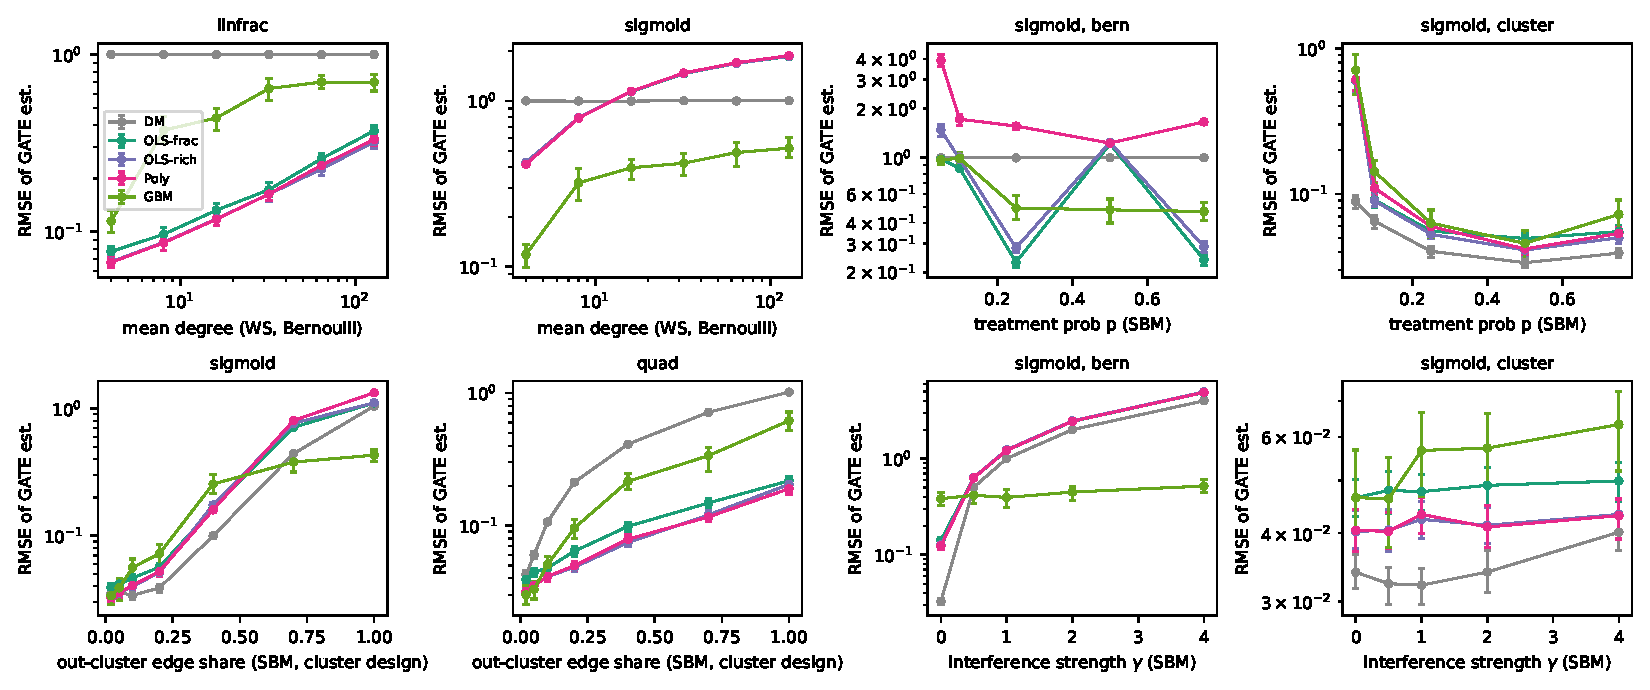
\includegraphics[width=\textwidth]{fig_sweeps.pdf}
\caption{RMSE (log scale, 95\% bootstrap intervals) of DM and regression estimators in sweeps. Top: mean degree (WS, Bernoulli; \texttt{linfrac}, \texttt{sigmoid}), treatment probability $p$ on SBM (Bernoulli, cluster; \texttt{sigmoid}). Bottom: out-cluster edge share $\rho$ of an SBM under cluster design (\texttt{sigmoid}, \texttt{quad}) and interference strength $\gamma$ (\texttt{sigmoid}; Bernoulli, cluster).}\label{fig:sweeps}\end{figure}

\textbf{E3/E6: variance of a correct model.} For \texttt{linfrac} on WS-Bernoulli, SD of OLS-frac/rich scales as $n^{-0.53}$ and $n^{-0.52}$ over $n\in[10^3,4\times10^4]$ (Fig.~\ref{fig:scaling}), and as $d^{0.46}$ and $d^{0.45}$ over $d\in[4,128]$ at $n=5000$: close to the $\sqrt{d/n}$ of the heuristic. The bias is within $\pm0.025$ (MC SE $\le0.02$). Hence the estimator is accurate but its \emph{sample size is effectively $n/d$}: at $d=128$ RMSE is 0.32--0.37. In contrast, for \texttt{sigmoid} the RMSE is flat in $n$ (1.28 $\to$ 1.24 for OLS-frac) since it is dominated by a constant bias (1.24--1.25); more data do not help.

\begin{figure}[t]\centering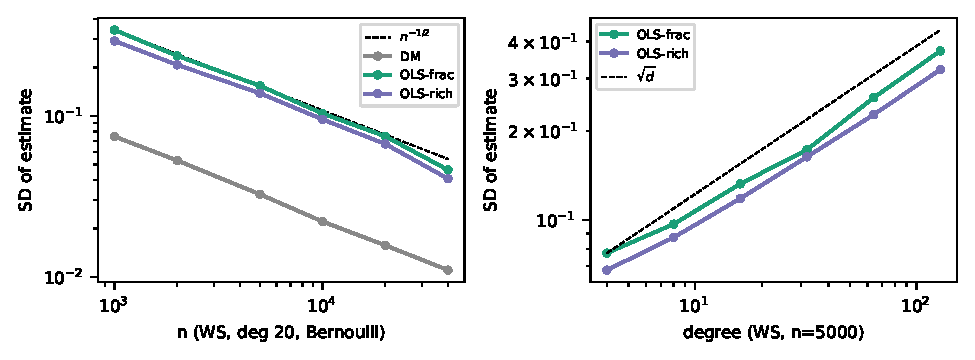
\includegraphics[width=.62\textwidth]{fig_scaling.pdf}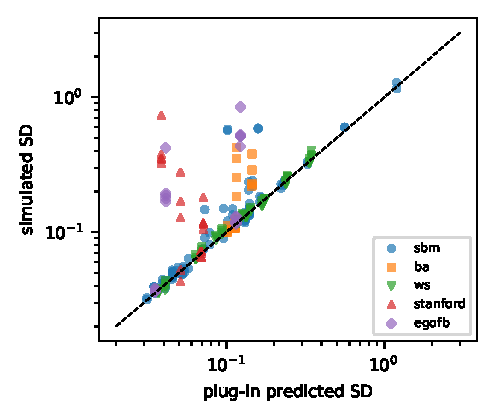
\includegraphics[width=.33\textwidth]{fig_predsd.pdf}
\caption{Left two: SD of the estimate vs.\ $n$ and degree (\texttt{linfrac}, WS, Bernoulli). Right: simulated SD vs.\ plug-in predicted SD over all configurations in E1--E5 (OLS-frac and OLS-rich; points above the line are underestimated by the heuristic).}\label{fig:scaling}\end{figure}

\textbf{Plug-in prediction (all E1--E5 configurations, 128 per estimator).} The ratio simulated SD/predicted SD for OLS-rich has median 1.01 (10--90\%: 0.94--1.27, max 5.4). For the correctly specified \texttt{linfrac} model on SBM and WS the ratio is 0.93--1.11 for OLS-frac and OLS-rich. The ratio is large where the iid-noise assumption breaks: configurations with few clusters (Stanford3: median ratio 3.2, up to 5.4; $p=0.05$ with 50 clusters: $\approx3.7$), where $\ell_i$-driven cluster-level residual variation and the small number of treated clusters add variance. OLS-frac omits $\ell$ whose variance (0.25) we add to $\sigma_e^2$; on real graphs the ratio is then 4--6, so omitted covariates correlated with graph position are costly (see coverage below).

\textbf{E2/E7: interference strength and noise.} For correctly specified models the error is independent of $\gamma$ (RMSE 0.12--0.15 across $\gamma\in[0,4]$ for linfrac, Bernoulli), while under \texttt{sigmoid}+Bernoulli the bias is $0.615,1.206,2.433,4.879$ for $\gamma=0.5,1,2,4$, i.e.\ $\approx1.2\gamma$ (Fig.~\ref{fig:sweeps}); with clusters it is $\le0.012$ for all $\gamma$. Noise scaling is linear (E7, linfrac: RMSE 0.031/0.141/0.506 for OLS-rich at $\sigma=0.25/1/4$).

\textbf{E4: treatment probability.} Under Bernoulli design the regressions have bias $-0.87,-0.77,-0.47,0.00,+0.49$ (\texttt{quad}, OLS-frac, $p=0.05,0.10,0.25,0.5,0.75$): the sign and size follow whether the observed $x\approx p$ lies on the same side of the curvature as the extrapolation targets; $p=0.5$ is accidentally best for \texttt{quad} (the quadratic's secant slope between $x=0.5$ and the targets happens to match the fitted slope) but worst for \texttt{sigmoid} (bias 1.21; at $p=0.25$ only $-0.15$). That the best $p$ flips sign across mechanisms shows that no $p$ is safe under misspecification. For cluster designs and $p\in[0.1,0.75]$ bias is $\le0.08$ but at $p=0.05$ (about 2.5 treated clusters of 50) SD is 0.57--0.58 and RMSE 0.60--0.63 (OLS-frac).

\textbf{E5: cluster quality.} On an SBM with cluster design, OLS-rich RMSE for \texttt{quad} increases smoothly from 0.032 ($\rho=0.02$) to 0.205 ($\rho=1$, i.e.\ clusters carry no information), and for \texttt{sigmoid} it is 0.033 at $\rho=0.02$, 0.051 at $0.2$, 0.17 at $0.4$ and 1.1 at $\rho=1$ with OLS-frac bias growing from 0.02 ($\rho=0.2$) to 1.08. For the linear-type mechanism the loss is variance (SD 0.039 $\to$ 0.218); the nonlinear \texttt{sigmoid} adds bias once $\rho\gtrsim0.4$. DM tracks the same pattern but is worse for \texttt{quad} throughout ($\rho=0.1$: 0.106 vs.\ 0.041).

\textbf{Interval coverage.} For correctly specified models (\texttt{linfrac}, \texttt{inter}) OLS-rich and Poly with HC1 intervals cover at 0.93--0.97 on all graphs and designs. OLS-frac, which omits the log-degree covariate that enters the outcome, covers at 0.94--0.97 on SBM/WS, but at 0.39 (Bernoulli) and 0.31--0.32 (cluster) on ego-FB, 0.86--0.87 / 0.17--0.18 on Stanford3, and 0.59 on BA-\texttt{inter}-cluster. We hypothesise (not tested) that, because $x_i$ and $x_j$ share treated neighbours while the omitted component is fixed, the independence assumption in the sandwich fails exactly when the omitted heterogeneity varies with graph position.

\textbf{Baselines.} Gradient boosting is best for \texttt{sigmoid} under Bernoulli on SBM/WS (0.42/0.45 vs.\ 1.2--1.3), because trees extrapolate as constants and the true response saturates; but for linear-type mechanisms GBM has RMSE 0.26--0.8 under Bernoulli, 2.5--5$\times$ worse than OLS-rich, and only $60$ repetitions were run. The Hajek exposure estimator is undefined in almost all Bernoulli draws on SBM, WS and Stanford3 (no unit has a fully treated and a fully control closed neighbourhood; shown as `--' in Appendix~B), is undefined in 9--14\% of draws on BA and well defined but noisy on ego-FB (RMSE 0.4--1.1, many weights near $p^{d+1}$). With clusters it is comparable to DM on SBM/WS (0.09--0.17) and about 2--3$\times$ worse than a correct regression; on BA with clusters it is undefined in up to 40\% of draws.

\section{Discussion and limitations}
\textbf{Answer to the question.} Where interference is one-hop and the regression family contains the truth, regression-based GATE estimation is accurate (RMSE $\approx0.04$--0.15 on a GATE of 2), and its error is governed by a design-leverage term $c^\top(X^\top X)^{-1}c$ that we can compute \emph{before} running the experiment. Where the family is wrong, the error is a bias that does not decay with $n$ and scales with $\gamma$; the experiment's own exposure support determines its size, and cluster randomization with good clusters is the most effective mitigation we found. The advice implied by our results is conditional on this simulation: prefer designs whose exposure support covers 0 and 1; report the leverage $c^\top(X^\top X)^{-1}c$ and the exposure distribution; do not trust nominal intervals when heterogeneity covariates are omitted; treat the number of clusters, not $n$, as sample size.

\textbf{Limitations.} (1) Outcomes are synthetic, one-hop and the graph is known and exact; two-hop interference, mis-measured edges and temporal effects are untested. (2) One graph draw per synthetic family, so graph-to-graph variability is not in the intervals; our statements about BA vs.\ SBM are about one instance each. (3) The \texttt{sigmoid} failure is partly by construction: we chose a response whose extrapolation from the observed support is hard, and the \texttt{quad} bias sign depends on curvature; numbers like ``$1.2\gamma$'' are specific to this function. (4) SBM clusters use the planted partition (oracle) while real graphs use Louvain, giving fewer clusters (10, 16) than ideal and confounding ``cluster quality'' with ``number of clusters''. (5) We do not evaluate the resampling-based inference or covariate-selection procedures of the cited regression-adjustment papers, only HC1 delta-method intervals; the interval conclusions do not transfer to them. (6) The plug-in prediction is heuristic, fails with few clusters, and we did not derive a corrected formula. (7) The explanation for the coverage failure is a hypothesis. (8) GBM was run with default-ish hyper-parameters and 60 repetitions. (9) No outcome-noise dependence across neighbours or spillover heterogeneity beyond the stated mechanisms was studied. (10) A first pass with $R=100$ (60$\to$20 GBM reps) used for debugging gave a qualitatively identical picture and was overwritten by the reported $R=300$ run; no configurations were dropped.

\bibliographystyle{plainnat}
\bibliography{refs}

\appendix
\section{Reproduction details}
Python 3.11, numpy 2.4.6, scipy 1.17.1, networkx 3.6.1, scikit-learn, pandas, matplotlib 3.11.2 (see \texttt{requirements.txt} in the code folder). Seeds: configuration $k$ in \texttt{run\_all.py} uses seed $k$ for assignment and noise; synthetic graphs use seed 1; Louvain seed 0. Total compute: roughly 12 minutes on 36 processes (single-threaded BLAS), no GPU. Scripts: \texttt{run\_all.py} $\to$ results JSON (E1--E7), \texttt{analyze.py} $\to$ Table~B (\texttt{tab\_main.tex}), Fig.~\ref{fig:sweeps}, Fig.~\ref{fig:scaling} (left) and coverage CSV, \texttt{maketab2.py} $\to$ Table~\ref{tab:small}, \texttt{predsd.py} $\to$ Fig.~\ref{fig:scaling} (right) and the plug-in statistics. Data: Stanford3 zip sha256 \texttt{b1221e41\ldots e8720d}, ego-Facebook sha256 \texttt{125e84db\ldots 35e}. Gradient-boosting settings: 150 iterations, learning rate 0.1. Bootstrap RMSE intervals: 200 resamples.

\section{Full RMSE table}
Columns: DM, OLS-frac, OLS-count, OLS-rich, Poly, GBM, Hajek. Bold is the smallest in the row; $\dagger$: estimator undefined in more than 5\% of draws; `--': undefined in nearly all draws. \texttt{inter} has $\tau_{\mathrm{GATE}}=3$.
\begin{table}[h]\centering\scriptsize\setlength{\tabcolsep}{3pt}
\begin{tabular}{lllccccccc}\toprule Graph & Mech. & Design & DM & Frac & Count & Rich & Poly & GBM & Hajek\\\midrule
SBM & linfrac & Bern & 1.00 & 0.14 & 1.76 & \textbf{0.13} & 0.13 & 0.52 & -- \\
SBM & linfrac & Clust & 0.10 & 0.05 & 0.16 & \textbf{0.04} & 0.04 & 0.05 & 0.10 \\
SBM & lincount & Bern & 1.00 & 0.16 & 2.21 & \textbf{0.12} & 0.13 & 0.52 & 2.91$^\dagger$ \\
SBM & lincount & Clust & 0.11 & 0.05 & 0.25 & \textbf{0.04} & 0.04 & 0.05 & 0.11 \\
SBM & quad & Bern & 1.00 & 0.15 & 1.75 & 0.13 & \textbf{0.12} & 0.46 & -- \\
SBM & quad & Clust & 0.11 & 0.05 & 0.16 & \textbf{0.04} & 0.04 & 0.04 & 0.10 \\
SBM & sigmoid & Bern & 1.00 & 1.22 & 2.44 & 1.23 & 1.22 & \textbf{0.42} & -- \\
SBM & sigmoid & Clust & \textbf{0.03} & 0.05 & 0.24 & 0.04 & 0.04 & 0.05 & 0.10 \\
SBM & inter & Bern & 1.50 & 0.13 & 1.53 & \textbf{0.12} & 0.12 & 0.73 & 1.52$^\dagger$ \\
SBM & inter & Clust & 0.15 & \textbf{0.04} & 0.12 & 0.04 & 0.04 & 0.05 & 0.09 \\
BA & linfrac & Bern & 1.00 & 0.11 & 0.26 & \textbf{0.10} & 0.10 & 0.26 & 1.04$^\dagger$ \\
BA & linfrac & Clust & 0.71 & \textbf{0.13} & 0.64 & 0.23 & 0.87 & 0.27 & 0.65$^\dagger$ \\
BA & lincount & Bern & 1.00 & 0.30 & 0.69 & \textbf{0.11} & 0.30 & 0.34 & 1.16$^\dagger$ \\
BA & lincount & Clust & 0.74 & 0.34 & 0.78 & \textbf{0.23} & 1.05 & 0.36 & 0.80$^\dagger$ \\
BA & quad & Bern & 1.00 & 0.11 & 0.27 & \textbf{0.10} & 0.10 & 0.31 & 1.02$^\dagger$ \\
BA & quad & Clust & 0.72 & 0.35 & 0.50 & 0.38 & 2.22 & \textbf{0.32} & 0.62$^\dagger$ \\
BA & sigmoid & Bern & 1.00 & 0.94 & \textbf{0.22} & 0.94 & 0.94 & 0.43 & 1.03$^\dagger$ \\
BA & sigmoid & Clust & 0.56 & 0.50 & 0.39 & 0.62 & 2.47 & \textbf{0.31} & 0.62$^\dagger$ \\
BA & inter & Bern & 1.50 & 0.11 & 0.74 & \textbf{0.10} & 0.10 & 0.39 & 0.94$^\dagger$ \\
BA & inter & Clust & 1.09 & 0.25 & 0.63 & \textbf{0.22} & 0.94 & 0.38 & 0.67$^\dagger$ \\
WS & linfrac & Bern & 1.00 & 0.15 & 1.19 & \textbf{0.13} & 0.13 & 0.49 & -- \\
WS & linfrac & Clust & 0.13 & \textbf{0.04} & 0.26 & 0.04 & 0.04 & 0.06 & 0.13 \\
WS & lincount & Bern & 1.00 & 0.15 & 1.26 & \textbf{0.13} & 0.13 & 0.51 & -- \\
WS & lincount & Clust & 0.14 & \textbf{0.04} & 0.29 & 0.04 & 0.04 & 0.07 & 0.15 \\
WS & quad & Bern & 1.00 & 0.14 & 1.18 & \textbf{0.13} & 0.13 & 0.52 & -- \\
WS & quad & Clust & 0.14 & \textbf{0.04} & 0.25 & 0.04 & 0.04 & 0.06 & 0.13 \\
WS & sigmoid & Bern & 1.00 & 1.26 & 2.32 & 1.26 & 1.27 & \textbf{0.45} & -- \\
WS & sigmoid & Clust & \textbf{0.04} & 0.06 & 0.31 & 0.06 & 0.05 & 0.06 & 0.15 \\
WS & inter & Bern & 1.50 & 0.14 & 1.14 & \textbf{0.13} & 0.13 & 0.68 & -- \\
WS & inter & Clust & 0.20 & \textbf{0.04} & 0.25 & 0.04 & 0.04 & 0.05 & 0.13 \\
Stanford3 & linfrac & Bern & 1.00 & 0.12 & 0.21 & \textbf{0.07} & 0.07 & 0.37 & -- \\
Stanford3 & linfrac & Clust & 0.44 & 0.38 & 0.47 & 0.28 & \textbf{0.13} & 0.15 & 0.43 \\
Stanford3 & lincount & Bern & 1.00 & 0.92 & 0.78 & \textbf{0.06} & 0.89 & 0.29 & -- \\
Stanford3 & lincount & Clust & 0.64 & 0.87 & 0.42 & \textbf{0.17} & 0.58 & 0.33 & 1.03 \\
Stanford3 & quad & Bern & 1.00 & 0.10 & 0.25 & 0.09 & \textbf{0.06} & 0.25 & -- \\
Stanford3 & quad & Clust & 0.46 & 0.35 & 0.17 & 0.13 & \textbf{0.12} & 0.13 & 0.43 \\
Stanford3 & sigmoid & Bern & 1.00 & 0.37 & \textbf{0.20} & 0.39 & 0.36 & 0.59 & -- \\
Stanford3 & sigmoid & Clust & 0.27 & 0.40 & 0.21 & 0.20 & \textbf{0.16} & 0.16 & 0.43 \\
Stanford3 & inter & Bern & 1.50 & 0.11 & 0.71 & \textbf{0.06} & 0.06 & 0.30 & -- \\
Stanford3 & inter & Clust & 0.68 & 0.32 & 0.33 & \textbf{0.04} & 0.04 & 0.15 & 0.47 \\
ego-FB & linfrac & Bern & 1.01 & 0.53 & 0.35 & \textbf{0.12} & 0.12 & 0.42 & 0.65 \\
ego-FB & linfrac & Clust & 0.18 & 0.19 & 0.11 & \textbf{0.04} & 0.04 & 0.06 & 0.28 \\
ego-FB & lincount & Bern & 1.00 & 1.13 & 0.65 & \textbf{0.13} & 0.77 & 0.38 & 1.10 \\
ego-FB & lincount & Clust & 0.40 & 0.42 & 0.10 & \textbf{0.04} & 0.19 & 0.06 & 0.64 \\
ego-FB & quad & Bern & 1.00 & 0.43 & 0.36 & 0.14 & \textbf{0.11} & 0.38 & 0.63 \\
ego-FB & quad & Clust & 0.17 & 0.17 & 0.10 & \textbf{0.04} & 0.04 & 0.05 & 0.27 \\
ego-FB & sigmoid & Bern & 1.00 & 0.81 & \textbf{0.32} & 0.62 & 0.63 & 0.55 & 0.65 \\
ego-FB & sigmoid & Clust & 0.18 & 0.19 & 0.11 & \textbf{0.04} & 0.04 & 0.06 & 0.30 \\
ego-FB & inter & Bern & 1.50 & 0.51 & 0.84 & \textbf{0.11} & 0.12 & 0.33 & 0.64 \\
ego-FB & inter & Clust & 0.18 & 0.18 & 0.10 & \textbf{0.04} & 0.04 & 0.05 & 0.27 \\
\bottomrule\end{tabular}\end{table}

\newpage
\section*{NeurIPS Paper Checklist}

\begin{enumerate}

\item {\bf Claims}
    \item[] Question: Do the main claims made in the abstract and introduction accurately reflect the paper's contributions and scope?
    \item[] Answer: \answerYes{}
    \item[] Justification: Abstract/intro claims are limited to the synthetic and Facebook-graph simulations reported in Sec.~4 and are qualified by the scope in Sec.~5.
    \item[] Guidelines:
    \begin{itemize}
        \item The answer NA means that the abstract and introduction do not include the claims made in the paper.
        \item The abstract and/or introduction should clearly state the claims made, including the contributions made in the paper and important assumptions and limitations. A No or NA answer to this question will not be perceived well by the reviewers. 
        \item The claims made should match theoretical and experimental results, and reflect how much the results can be expected to generalize to other settings. 
        \item It is fine to include aspirational goals as motivation as long as it is clear that these goals are not attained by the paper. 
    \end{itemize}

\item {\bf Limitations}
    \item[] Question: Does the paper discuss the limitations of the work performed by the authors?
    \item[] Answer: \answerYes{}
    \item[] Justification: Sec.~5 (Limitations) lists the main ones: single graph realisation per synthetic family, one-hop interference only, correctly specified neighbourhood graph, oracle clusters for SBM.
    \item[] Guidelines:
    \begin{itemize}
        \item The answer NA means that the paper has no limitation while the answer No means that the paper has limitations, but those are not discussed in the paper. 
        \item The authors are encouraged to create a separate "Limitations" section in their paper.
        \item The paper should point out any strong assumptions and how robust the results are to violations of these assumptions (e.g., independence assumptions, noiseless settings, model well-specification, asymptotic approximations only holding locally). The authors should reflect on how these assumptions might be violated in practice and what the implications would be.
        \item The authors should reflect on the scope of the claims made, e.g., if the approach was only tested on a few datasets or with a few runs. In general, empirical results often depend on implicit assumptions, which should be articulated.
        \item The authors should reflect on the factors that influence the performance of the approach. For example, a facial recognition algorithm may perform poorly when image resolution is low or images are taken in low lighting. Or a speech-to-text system might not be used reliably to provide closed captions for online lectures because it fails to handle technical jargon.
        \item The authors should discuss the computational efficiency of the proposed algorithms and how they scale with dataset size.
        \item If applicable, the authors should discuss possible limitations of their approach to address problems of privacy and fairness.
        \item While the authors might fear that complete honesty about limitations might be used by reviewers as grounds for rejection, a worse outcome might be that reviewers discover limitations that aren't acknowledged in the paper. The authors should use their best judgment and recognize that individual actions in favor of transparency play an important role in developing norms that preserve the integrity of the community. Reviewers will be specifically instructed to not penalize honesty concerning limitations.
    \end{itemize}

\item {\bf Theory assumptions and proofs}
    \item[] Question: For each theoretical result, does the paper provide the full set of assumptions and a complete (and correct) proof?
    \item[] Answer: \answerNA{}
    \item[] Justification: No theorems; the variance expression in Sec.~3 is a heuristic plug-in approximation that is checked empirically, not claimed as a theorem.
    \item[] Guidelines:
    \begin{itemize}
        \item The answer NA means that the paper does not include theoretical results. 
        \item All the theorems, formulas, and proofs in the paper should be numbered and cross-referenced.
        \item All assumptions should be clearly stated or referenced in the statement of any theorems.
        \item The proofs can either appear in the main paper or the supplemental material, but if they appear in the supplemental material, the authors are encouraged to provide a short proof sketch to provide intuition. 
        \item Inversely, any informal proof provided in the core of the paper should be complemented by formal proofs provided in appendix or supplemental material.
        \item Theorems and Lemmas that the proof relies upon should be properly referenced. 
    \end{itemize}

    \item {\bf Experimental result reproducibility}
    \item[] Question: Does the paper fully disclose all the information needed to reproduce the main experimental results of the paper to the extent that it affects the main claims and/or conclusions of the paper (regardless of whether the code and data are provided or not)?
    \item[] Answer: \answerYes{}
    \item[] Justification: Sec.~3--4 and Appendix~A describe graphs, outcome models, designs, estimators, parameters; all code is in the supplementary code with a README.
    \item[] Guidelines:
    \begin{itemize}
        \item The answer NA means that the paper does not include experiments.
        \item If the paper includes experiments, a No answer to this question will not be perceived well by the reviewers: Making the paper reproducible is important, regardless of whether the code and data are provided or not.
        \item If the contribution is a dataset and/or model, the authors should describe the steps taken to make their results reproducible or verifiable. 
        \item Depending on the contribution, reproducibility can be accomplished in various ways. For example, if the contribution is a novel architecture, describing the architecture fully might suffice, or if the contribution is a specific model and empirical evaluation, it may be necessary to either make it possible for others to replicate the model with the same dataset, or provide access to the model. In general. releasing code and data is often one good way to accomplish this, but reproducibility can also be provided via detailed instructions for how to replicate the results, access to a hosted model (e.g., in the case of a large language model), releasing of a model checkpoint, or other means that are appropriate to the research performed.
        \item While NeurIPS does not require releasing code, the conference does require all submissions to provide some reasonable avenue for reproducibility, which may depend on the nature of the contribution. For example
        \begin{enumerate}
            \item If the contribution is primarily a new algorithm, the paper should make it clear how to reproduce that algorithm.
            \item If the contribution is primarily a new model architecture, the paper should describe the architecture clearly and fully.
            \item If the contribution is a new model (e.g., a large language model), then there should either be a way to access this model for reproducing the results or a way to reproduce the model (e.g., with an open-source dataset or instructions for how to construct the dataset).
            \item We recognize that reproducibility may be tricky in some cases, in which case authors are welcome to describe the particular way they provide for reproducibility. In the case of closed-source models, it may be that access to the model is limited in some way (e.g., to registered users), but it should be possible for other researchers to have some path to reproducing or verifying the results.
        \end{enumerate}
    \end{itemize}


\item {\bf Open access to data and code}
    \item[] Question: Does the paper provide open access to the data and code, with sufficient instructions to faithfully reproduce the main experimental results, as described in supplemental material?
    \item[] Answer: \answerYes{}
    \item[] Justification: Code and seeds are provided; the two graphs are public (URLs, hashes in README). Commands are in README.
    \item[] Guidelines:
    \begin{itemize}
        \item The answer NA means that paper does not include experiments requiring code.
        \item Please see the NeurIPS code and data submission guidelines (\url{https://nips.cc/public/guides/CodeSubmissionPolicy}) for more details.
        \item While we encourage the release of code and data, we understand that this might not be possible, so “No” is an acceptable answer. Papers cannot be rejected simply for not including code, unless this is central to the contribution (e.g., for a new open-source benchmark).
        \item The instructions should contain the exact command and environment needed to run to reproduce the results. See the NeurIPS code and data submission guidelines (\url{https://nips.cc/public/guides/CodeSubmissionPolicy}) for more details.
        \item The authors should provide instructions on data access and preparation, including how to access the raw data, preprocessed data, intermediate data, and generated data, etc.
        \item The authors should provide scripts to reproduce all experimental results for the new proposed method and baselines. If only a subset of experiments are reproducible, they should state which ones are omitted from the script and why.
        \item At submission time, to preserve anonymity, the authors should release anonymized versions (if applicable).
        \item Providing as much information as possible in supplemental material (appended to the paper) is recommended, but including URLs to data and code is permitted.
    \end{itemize}


\item {\bf Experimental setting/details}
    \item[] Question: Does the paper specify all the training and test details (e.g., data splits, hyperparameters, how they were chosen, type of optimizer, etc.) necessary to understand the results?
    \item[] Answer: \answerYes{}
    \item[] Justification: Sec.~4 and Appendix~A give all parameters (n, degrees, p, gamma, sigma, repetitions, GBM settings).
    \item[] Guidelines:
    \begin{itemize}
        \item The answer NA means that the paper does not include experiments.
        \item The experimental setting should be presented in the core of the paper to a level of detail that is necessary to appreciate the results and make sense of them.
        \item The full details can be provided either with the code, in appendix, or as supplemental material.
    \end{itemize}

\item {\bf Experiment statistical significance}
    \item[] Question: Does the paper report error bars suitably and correctly defined or other appropriate information about the statistical significance of the experiments?
    \item[] Answer: \answerYes{}
    \item[] Justification: RMSE bootstrap 95\% intervals (Fig.~1, Appendix tables in the released JSON), Monte-Carlo SE of bias, and empirical coverage of CIs; 300 repetitions per configuration (60 for GBM).
    \item[] Guidelines:
    \begin{itemize}
        \item The answer NA means that the paper does not include experiments.
        \item The authors should answer "Yes" if the results are accompanied by error bars, confidence intervals, or statistical significance tests, at least for the experiments that support the main claims of the paper.
        \item The factors of variability that the error bars are capturing should be clearly stated (for example, train/test split, initialization, random drawing of some parameter, or overall run with given experimental conditions).
        \item The method for calculating the error bars should be explained (closed form formula, call to a library function, bootstrap, etc.)
        \item The assumptions made should be given (e.g., Normally distributed errors).
        \item It should be clear whether the error bar is the standard deviation or the standard error of the mean.
        \item It is OK to report 1-sigma error bars, but one should state it. The authors should preferably report a 2-sigma error bar than state that they have a 96\% CI, if the hypothesis of Normality of errors is not verified.
        \item For asymmetric distributions, the authors should be careful not to show in tables or figures symmetric error bars that would yield results that are out of range (e.g. negative error rates).
        \item If error bars are reported in tables or plots, The authors should explain in the text how they were calculated and reference the corresponding figures or tables in the text.
    \end{itemize}

\item {\bf Experiments compute resources}
    \item[] Question: For each experiment, does the paper provide sufficient information on the computer resources (type of compute workers, memory, time of execution) needed to reproduce the experiments?
    \item[] Answer: \answerYes{}
    \item[] Justification: Appendix~A: about 15 minutes of wall-clock on a 40-core CPU for all experiments; no GPU.
    \item[] Guidelines:
    \begin{itemize}
        \item The answer NA means that the paper does not include experiments.
        \item The paper should indicate the type of compute workers CPU or GPU, internal cluster, or cloud provider, including relevant memory and storage.
        \item The paper should provide the amount of compute required for each of the individual experimental runs as well as estimate the total compute. 
        \item The paper should disclose whether the full research project required more compute than the experiments reported in the paper (e.g., preliminary or failed experiments that didn't make it into the paper). 
    \end{itemize}
    
\item {\bf Code of ethics}
    \item[] Question: Does the research conducted in the paper conform, in every respect, with the NeurIPS Code of Ethics \url{https://neurips.cc/public/EthicsGuidelines}?
    \item[] Answer: \answerYes{}
    \item[] Justification: The research uses only synthetic outcomes and public graphs and follows the NeurIPS Code of Ethics.
    \item[] Guidelines:
    \begin{itemize}
        \item The answer NA means that the authors have not reviewed the NeurIPS Code of Ethics.
        \item If the authors answer No, they should explain the special circumstances that require a deviation from the Code of Ethics.
        \item The authors should make sure to preserve anonymity (e.g., if there is a special consideration due to laws or regulations in their jurisdiction).
    \end{itemize}


\item {\bf Broader impacts}
    \item[] Question: Does the paper discuss both potential positive societal impacts and negative societal impacts of the work performed?
    \item[] Answer: \answerNA{}
    \item[] Justification: Methodological/simulation study without deployment; no direct societal impact beyond general A/B-testing practice.
    \item[] Guidelines:
    \begin{itemize}
        \item The answer NA means that there is no societal impact of the work performed.
        \item If the authors answer NA or No, they should explain why their work has no societal impact or why the paper does not address societal impact.
        \item Examples of negative societal impacts include potential malicious or unintended uses (e.g., disinformation, generating fake profiles, surveillance), fairness considerations (e.g., deployment of technologies that could make decisions that unfairly impact specific groups), privacy considerations, and security considerations.
        \item The conference expects that many papers will be foundational research and not tied to particular applications, let alone deployments. However, if there is a direct path to any negative applications, the authors should point it out. For example, it is legitimate to point out that an improvement in the quality of generative models could be used to generate deepfakes for disinformation. On the other hand, it is not needed to point out that a generic algorithm for optimizing neural networks could enable people to train models that generate Deepfakes faster.
        \item The authors should consider possible harms that could arise when the technology is being used as intended and functioning correctly, harms that could arise when the technology is being used as intended but gives incorrect results, and harms following from (intentional or unintentional) misuse of the technology.
        \item If there are negative societal impacts, the authors could also discuss possible mitigation strategies (e.g., gated release of models, providing defenses in addition to attacks, mechanisms for monitoring misuse, mechanisms to monitor how a system learns from feedback over time, improving the efficiency and accessibility of ML).
    \end{itemize}
    
\item {\bf Safeguards}
    \item[] Question: Does the paper describe safeguards that have been put in place for responsible release of data or models that have a high risk for misuse (e.g., pretrained language models, image generators, or scraped datasets)?
    \item[] Answer: \answerNA{}
    \item[] Justification: No models or scraped data with misuse risk are released.
    \item[] Guidelines:
    \begin{itemize}
        \item The answer NA means that the paper poses no such risks.
        \item Released models that have a high risk for misuse or dual-use should be released with necessary safeguards to allow for controlled use of the model, for example by requiring that users adhere to usage guidelines or restrictions to access the model or implementing safety filters. 
        \item Datasets that have been scraped from the Internet could pose safety risks. The authors should describe how they avoided releasing unsafe images.
        \item We recognize that providing effective safeguards is challenging, and many papers do not require this, but we encourage authors to take this into account and make a best faith effort.
    \end{itemize}

\item {\bf Licenses for existing assets}
    \item[] Question: Are the creators or original owners of assets (e.g., code, data, models), used in the paper, properly credited and are the license and terms of use explicitly mentioned and properly respected?
    \item[] Answer: \answerYes{}
    \item[] Justification: Stanford3 (Traud et al. 2012; Network Repository, CC BY-SA) and SNAP ego-Facebook (McAuley \& Leskovec 2012) are cited; versions/hashes in README.
    \item[] Guidelines:
    \begin{itemize}
        \item The answer NA means that the paper does not use existing assets.
        \item The authors should cite the original paper that produced the code package or dataset.
        \item The authors should state which version of the asset is used and, if possible, include a URL.
        \item The name of the license (e.g., CC-BY 4.0) should be included for each asset.
        \item For scraped data from a particular source (e.g., website), the copyright and terms of service of that source should be provided.
        \item If assets are released, the license, copyright information, and terms of use in the package should be provided. For popular datasets, \url{paperswithcode.com/datasets} has curated licenses for some datasets. Their licensing guide can help determine the license of a dataset.
        \item For existing datasets that are re-packaged, both the original license and the license of the derived asset (if it has changed) should be provided.
        \item If this information is not available online, the authors are encouraged to reach out to the asset's creators.
    \end{itemize}

\item {\bf New assets}
    \item[] Question: Are new assets introduced in the paper well documented and is the documentation provided alongside the assets?
    \item[] Answer: \answerYes{}
    \item[] Justification: The released code and the README are new assets; no new datasets.
    \item[] Guidelines:
    \begin{itemize}
        \item The answer NA means that the paper does not release new assets.
        \item Researchers should communicate the details of the dataset/code/model as part of their submissions via structured templates. This includes details about training, license, limitations, etc. 
        \item The paper should discuss whether and how consent was obtained from people whose asset is used.
        \item At submission time, remember to anonymize your assets (if applicable). You can either create an anonymized URL or include an anonymized zip file.
    \end{itemize}

\item {\bf Crowdsourcing and research with human subjects}
    \item[] Question: For crowdsourcing experiments and research with human subjects, does the paper include the full text of instructions given to participants and screenshots, if applicable, as well as details about compensation (if any)? 
    \item[] Answer: \answerNA{}
    \item[] Justification: No crowdsourcing or human subjects.
    \item[] Guidelines:
    \begin{itemize}
        \item The answer NA means that the paper does not involve crowdsourcing nor research with human subjects.
        \item Including this information in the supplemental material is fine, but if the main contribution of the paper involves human subjects, then as much detail as possible should be included in the main paper. 
        \item According to the NeurIPS Code of Ethics, workers involved in data collection, curation, or other labor should be paid at least the minimum wage in the country of the data collector. 
    \end{itemize}

\item {\bf Institutional review board (IRB) approvals or equivalent for research with human subjects}
    \item[] Question: Does the paper describe potential risks incurred by study participants, whether such risks were disclosed to the subjects, and whether Institutional Review Board (IRB) approvals (or an equivalent approval/review based on the requirements of your country or institution) were obtained?
    \item[] Answer: \answerNA{}
    \item[] Justification: No human subjects.
    \item[] Guidelines:
    \begin{itemize}
        \item The answer NA means that the paper does not involve crowdsourcing nor research with human subjects.
        \item Depending on the country in which research is conducted, IRB approval (or equivalent) may be required for any human subjects research. If you obtained IRB approval, you should clearly state this in the paper. 
        \item We recognize that the procedures for this may vary significantly between institutions and locations, and we expect authors to adhere to the NeurIPS Code of Ethics and the guidelines for their institution. 
        \item For initial submissions, do not include any information that would break anonymity (if applicable), such as the institution conducting the review.
    \end{itemize}

\item {\bf Declaration of LLM usage}
    \item[] Question: Does the paper describe the usage of LLMs if it is an important, original, or non-standard component of the core methods in this research? Note that if the LLM is used only for writing, editing, or formatting purposes and does not impact the core methodology, scientific rigorousness, or originality of the research, declaration is not required.
    %this research? 
    \item[] Answer: \answerNA{}
    \item[] Justification: LLMs are not a component of the method (classical regression estimators). An LLM coding assistant helped write code and text; all reported numbers come from the released code.
    \item[] Guidelines:
    \begin{itemize}
        \item The answer NA means that the core method development in this research does not involve LLMs as any important, original, or non-standard components.
        \item Please refer to our LLM policy (\url{https://neurips.cc/Conferences/2025/LLM}) for what should or should not be described.
    \end{itemize}

\end{enumerate}


\end{document}
\end{document}
